\chapter{I filtri di Bloom}

\section{Strutture dati e algoritmi probabilistici}

Le strutture dati e gli algoritmi che basano il proprio funzionamento sull'utilizzo di una componente
di casualità vengono detti ``probabilistici''. 

Ci sono due principali famiglie di algoritmi probabilistici:

\begin{itemize}
	\medskip

	\item Gli algoritmi detti ``Monte Carlo'', nei quali si effettua un campionamento casuale di
	valori in uno spazio di ricerca, consentendo il calcolo approssimato entro una certa
	probabilità. Il nome deriva dal Principato di Monte Carlo, conosciuto a livello mondiale come
	meta per il gioco d'azzardo. Gli algoritmi di questo tipo permettono solitamente di bilanciare
	il tempo di esecuzione con l'errore richiesto, poiché aumentando il numero di tentativi l'errore
	scende. Un esempio di questi algoritmi sono i test di primalità (cioè i test per verificare se
	un numero è primo) come il test di Fermat, nei quali si effettua controlli di una condizione
	necessaria ma non sufficiente e ci si convince che il numero è il primo quando con un
	determinato numero di tentativi.

	\item Gli algoritmi detti ``Las Vegas'', nei quali si utilizza la casualità durante l'algoritmo,
	ma viene prodotto sempre un risultato esatto, oppure l'algoritmo fallisce esplicitamente
	l'esecuzione. In questo caso dunque la componente casuale non è parte integrante della qualità
	risultato ottenuto, ma può influenzare il tempo d'esecuzione. Un esempio classico è l'algoritmo
	di ordinamento ``Quicksort'' in cui la scelta del pivot da utilizzare ad ogni passaggio è
	casuale, ma il risultato è sempre corretto. Il nome è stato proposto in \cite{lasvegas} per
	contrasto con Monte Carlo, dato che Las Vegas è un'altra meta conosciuta per il gioco d'azzardo.
\end{itemize}

Nelle strutture dati, invece, l'utilizzo del caso permette la memorizzazione di un'informazione
parziale, consentendo comunque di elaborarla almeno parzialmente ma con margini di errori
accettabili. Si tratta tipicamente di strutture dati molto specialistiche, utili ad implementare un
solo specifico algoritmo, poiché la perdita di informazione controllata è orientata a memorizzare il
minimo indispensabile per lo specifico scenario d'uso, ma impedendo ovviamente delle operazioni che
richiedono l'informazione completa, come anche la semplice enumerazione.

\section{Gli insiemi}

Un insieme è una struttura dati che memorizza un gruppo di elementi distinti, senza alcun ordine tra
essi (quindi né ordinamento intrinseco dei dati, né ordinamento esterno quale per esempio l'ordine
di inserimento).

Le operazioni principali che si possono effettuare sulla struttura dati sono le seguenti:

\begin{itemize}
	\medskip

	\item
	\textbf{Inserimento}: aggiunge un elemento all'insieme. Se l'elemento è già presente,
	l'operazione non modifica la struttura dati. In alcune implementazioni, l'operazione può 
	restituire un codice di errore per indicare che l'inserimento non è stato effettuato
	perché l'elemento era già presente.

	\item
	\textbf{Test di appartenenza}: controlla se un elemento è presente nell'insieme.

	\item
	\textbf{Cardinalità}: restituisce il numero di elementi presenti nell'insieme.

	\item
	\textbf{Unione}: restituisce un insieme che contiene tutti gli elementi presenti in almeno uno
	degli insiemi forniti in ingresso.

	\item
	\textbf{Intersezione}: restituisce un insieme che contiene tutti gli elementi presenti in tutti
	gli insiemi forniti in ingresso.
\end{itemize}

Alcune implementazioni offrono anche operazioni più avanzate legate alla teoria degli insiemi,
come per esempio la differenza o la differenza simmetrica. 

Un'implementazione classica di un'insieme prevede l'utilizzo di una tabella hash: l'inserimento
di un elemento avviene codificandolo con una funzione hash, memorizzandolo all'interno della
tabella, gestendo in modo opportuno le collisioni; il test di appartenenza può essere fatto così in
modo efficiente effettuando una ricerca nella tabella hash. Entrambe queste operazioni così 
implementate richiedono quindi un tempo d'esecuzione ammortizzato costante (\verb|O(k)|).

Al contrario di un array associativo, un insieme non ha dati associati all'elemento stesso, ma
nonostante questo è spesso possibile riutilizzare la stessa implementazione di tabella hash,
associando un dato nullo (non significativo) all'elemento. Questo accade comunemente nei linguaggi e
nelle librerie che mettono a disposizione una struttura dati di tipo array associativo (poiché più
completa); per esempio, il linguaggio Python fin dalla versione 1.0 prevedeva il ``dizionario'' come
struttura dati (un array associativo implementato con tabella hash), mentre l'``insieme'' è stato
aggiunto nella versione 2.3; prima di allora, era comune implementare l'insieme con un dizionario i
cui valori erano semplicemente valori booleani (di solito \verb|True|).

\section{Propriet\`a dei filtri di Bloom}

Un filtro di Bloom è una rappresentazione probabilistica di un insieme. Nel filtro infatti
non vengono memorizzati per intero tutti gli elementi, ma ne viene memorizzata solo una
rappresentazione parziale, che consente di effettuare comunque alcune operazioni, mantenendo però
dei margini di errore controllati. 

In particolare, il test di appartenenza restituisce un valore probabilistico, con la presenza di
falsi valori positivi (cioè il test restituisce un valore di successo anche per elementi non
effettivamente presenti). Il margine di errore può essere controllato tramite alcuni parametri, che
vengono stabiliti al momento della creazione del filtro stesso.

Vediamo nel dettaglio come i filtri si comportano relativamente alle operazioni principali sugli
insiemi elencate precedentemente:

\begin{itemize}
	\medskip

	\item
	\textbf{Inserimento}: è possibile inserire un elemento in un filtro, fino ad un numero massimo
	di elementi calcolabile in base ai parametri del filtro stesso. I filtri non possono essere
	infatti ridimensionati dopo la creazione e quando raggiungono il numero massimo di elementi,
	l'aggiunta di ulteriori elementi, seppure tecnicamente possibile, aumenta esponenzialmente 
	il margine di errore, rendendo di fatto il filtro inutilizzabile.

	Durante l'inserimento, è possibile effettuare contemporaneamente un test di appartenenza,
	restituendo una informazione probabilistica se l'elemento inserito era già presente o meno.

	\item
	\textbf{Test di appartenenza}: il filtro è in grado di verificare se un elemento è stato
	inserito con un certo margine di errore. In particolare, se il test restituisce un valore
	positivo, l'elemento è \emph{probabilmente presente}, con una soglia di errore controllato;
	ciò vuol dire che non si può avere la certezza che l'elemento sia effettivamente presente
	nell'insieme. Viceversa, se il test restituisce un valore negativo, si ha la certezza che il
	valore non è presente nell'insieme.

	\item
	\textbf{Cardinalità}: il filtro è in grado di effettuare una stima della cardinalità, compiendo
	un errore controllato sul valore restituito. I risultati rimangono consistenti anche al crescere
	della densità.

	\item
	\textbf{Unione}: è possibile calcolare con precisione l'unione di due filtri, purché siano
	creati con gli stessi parametri. Si noti che l'unione risultante dovrà rispettare il limite
	massimo di elementi previsto dai parametri di creazione, altrimenti non sarà utilizzabile.

	\item
	\textbf{Intersezione}: è possibile calcolare con precisione l'intersezione di due filtri,
	purché siano creati con gli stessi parametri.

\end{itemize}

\section{Funzionamento dei filtri}

Un filtro di Bloom è un array di bit, utilizzato come tabella hash, di dimensione arbitraria
\verb|M| fissata al momento della creazione in base ai parametri (vedi \ref{sec:bloomparms}).
Quando il filtro è vuoto, tutti i bit sono impostati a 0.

L'inserimento di un elemento $X$ avviene calcolando alcune funzioni di hash $h_i(X)$ prestabilite
sull'elemento (il numero delle funzioni, chiamato $K$, è anch'esso un parametro del filtro). I $K$
valori risultanti $h_0(X), h_1(X), ... , h_K(X)$ sono utilizzati per identificare singoli bit
all'interno dell'array (per esempio, scegliendo il bit con indice $h_i(X) \bmod M$), e i bit così
identificati vengono impostati a 1. Si noti che nessuna altra informazione sull'elemento viene
memorizzata dentro il filtro.

Il test di appartenenza di un elemento segue un processo simmetrico: vengono eseguite le \verb|K|
funzioni di hash e si identificano così \verb|K| bit dell'array. Se tutti i bit sono impostati a 1,
l'elemento è \emph{probabilmente presente} all'interno del filtro; se almeno uno dei bit è
impostato a 0, l'elemento è \emph{sicuramente assente} all'interno del filtro.

Il motivo per cui il test di appartenenza non può asserire con certezza la presenza di un elemento
è dovuto all'assenza di un meccanismo di rilevamento delle collisioni delle funzioni di hash tra
elementi distinti; quando il test verifica se un determinato bit è impostato a 1, non può sapere
se quel bit è stato impostato tramite l'inserimento dell'elemento su cui si sta effettuando il test,
o tramite l'inserimento di un altro elemento che è in conflitto a livello di funzione di hash. Se
un elemento che non è presente utilizza, per il test di primalità, \verb|K| bit che sono stati
precedenti accesi da altri elementi tramite le varie funzioni di hash ad essi applicate, l'elemento
risulterà falsamente presente nel filtro, causando un cosiddetto \emph{falso positivo}.  

\subsection{Scelta delle funzioni di hash}

Utilizzo del double-hashing come metodo efficiente
Utilizzo del partizionamento in sezioni

Dillinger, Peter C.; Manolios, Panagiotis (2004b), "Bloom Filters in Probabilistic Verification", Proceedings of the 5th International Conference on Formal Methods in Computer-Aided Design, Springer-Verlag, Lecture Notes in Computer Science 3312


\subsection{Stima della cardinalità}
\label{sec:bloomcard}

È possibile effettuare una stima della cardinalità \verb|N| di un filtro di Bloom, derivandola
dalla densità, come già mostrato in \cite{bloomcard} \cite{bloomscalable}.

Si noti che un filtro di dimensione $M$ con $K$ funzioni di hash può essere implementato, senza
perdita di genericità, con $K$ array distinti di $m=\frac{M}{K}$ bit ciascuno, chiamati
\emph{sezioni}; in questo caso, le funzioni di hash dovranno essere utilizzate per indicizzare
ciascuno un bit all'interno di una sezione distinta, utilizzando per esempio $h_i(X) \bmod m$.

Ciascuna sezione inizia il ciclo di vita con tutti i bit impostati a 0. Dopo l'inserimento di un
elemento nel filtro, un solo bit sarà stato impostati a 1, per cui la probabilità $p$ che un bit
della sezione sia impostato a 1 (detta anche \emph{densità}) è $\frac{1}{m}$, mentre la probabilità
$q$ che un bit sia impostato a 0 è $ q=1-\frac{1}{m}$. Dopo $n$ inserimenti, le probabilità saranno
quindi: 

$$ q = (1-\frac{1}{m})^n $$
$$ p = 1-(1-\frac{1}{m})^n $$

Per ricavare $n$, si ricordi la seguente serie di Taylor:

$$ e^{-\frac{1}{x}} = 1 - \frac{1}{x} + \mathcal{O}((\frac{1}{x})^2) $$

dal quale si deriva:

$$ p \approx 1-(e^{-\frac{1}{m}})^n $$
$$ \ln(1-p) \approx -\frac{n}{m} $$
$$ n \approx -m\ln(1-p) $$
$$ n \approx -\frac{M}{K}\ln(1-p) $$

che è possibile valutare quindi estraendo la densità $p$ del filtro da un semplice conteggio
dei bit impostati ad 1 in un dato momento.

I seguenti grafici mostrano l'errore di calcolo della cardinalità effettuato in un filtro al crescere
della densità, e al numero di funzioni di hash. Come si può vedere, l'errore effettuato dalla stima
non diverge anche per valori di densità elevati.

\begin{figure}
	\centering

	\begin{subfigure}[t]{280px}
	\centering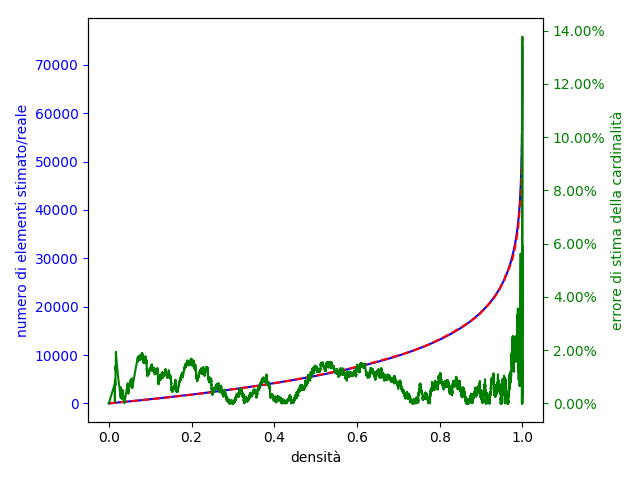
\includegraphics[width=280px]{bloom_card_error_1h}
	\subcaption{M=8192, K=1}
	\end{subfigure}

	\begin{subfigure}[t]{280px}
	\centering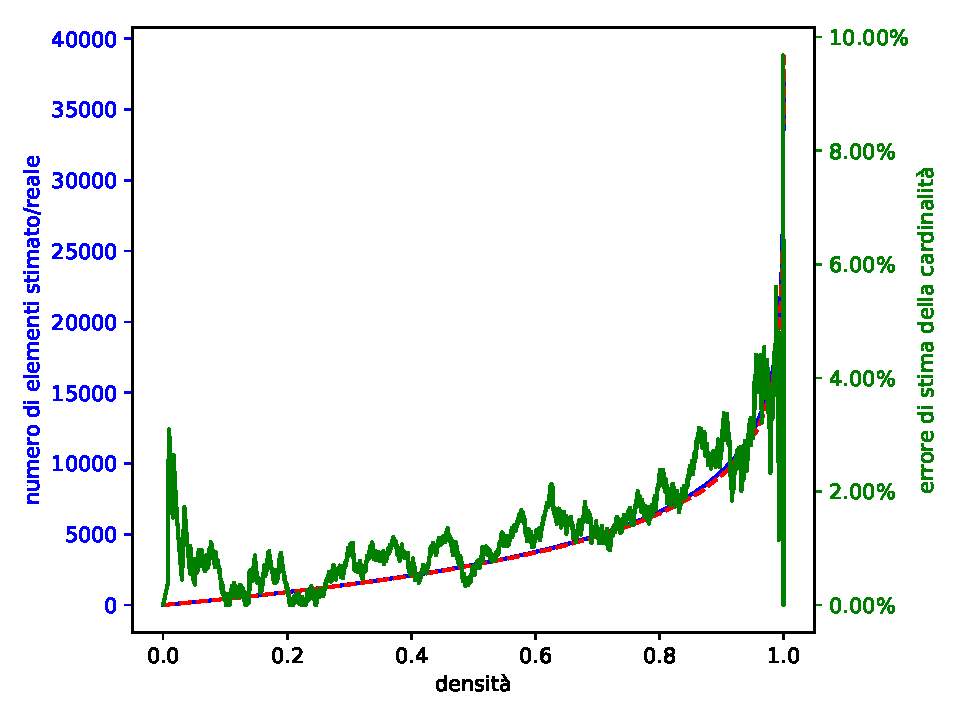
\includegraphics[width=280px]{bloom_card_error_2h}
	\subcaption{M=8192, K=2}
	\end{subfigure}

	\begin{subfigure}[t]{280px}
	\centering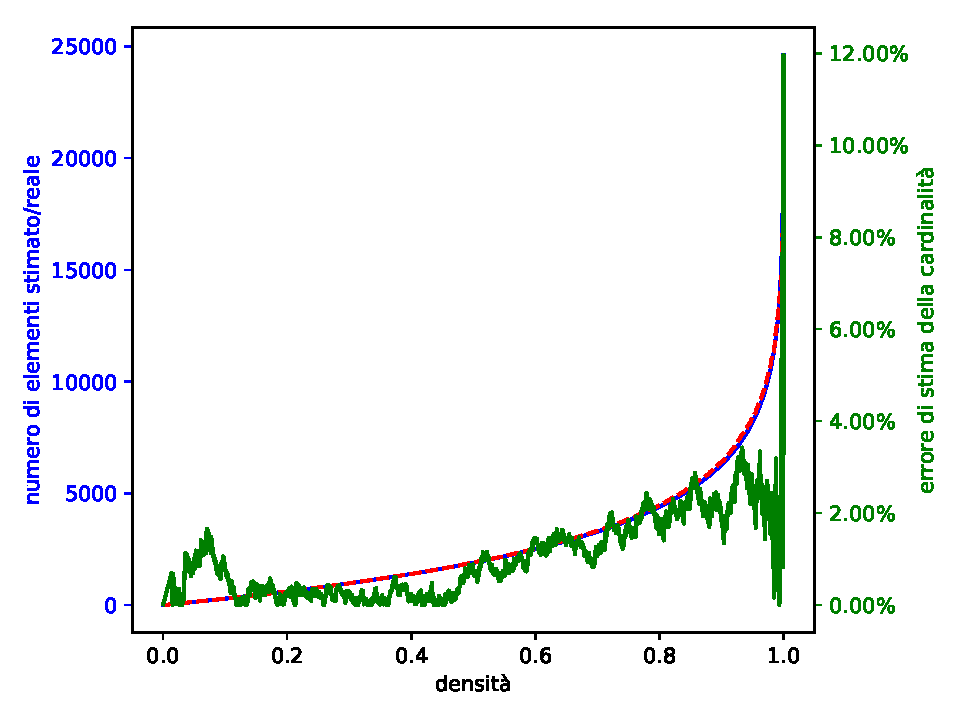
\includegraphics[width=280px]{bloom_card_error_3h}
	\subcaption{M=8192, K=3}
	\end{subfigure}

	\caption{Errore sulla cardinalità nei filtri di Bloom}
\end{figure}


\section{Ottimizzazione dei parametri}
\label{sec:bloomparms}

Ci sono diversi parametri di interesse quando si analizza un filtro di Bloom, riassunti in questa
tabella.

\medskip
\begin{tabular}{ |l|l| }
  \hline
  \multicolumn{2}{|c|}{Parametri} \\
  \hline
  $M$ & Dimensione in bit dell'array \\
  $K$ & Numero delle funzioni di hash (e delle sezioni) \\
  $m$ & Dimensione in bit di una sezione \\
  $N$ & Numero di elementi presenti nel filtro \\
  $p$ & Densità \\
  $P$ & Probabilità di un falso positivo \\
  \hline
\end{tabular}

\medskip

Vediamo ora come è possibile ottimizzare i parametri, cercando di minimizzare $P$, la probabilità
di un falso positivo, come descritto in \cite{bloomscalable}.

La probabilità di trovare un bit impostato a 1 in una sezione è $p$, di conseguenza la probabilità 
di un falso positivo, cioè di trovare i bit di tutte le sezioni già impostati, è:

$$ P = p^K $$

Ricordando che $M=km$, otteniamo:

$$ m = M\frac{\ln(p)}{\ln(P)} $$

e sostituendo nella formula della cardinalità, otteniamo:

$$ N \approx -M\frac{\ln(p)\ln(1-p)}{\ln(P)} $$

Supponiamo ora di fissare $M$ (dimensione del filtro) e $P$ (probabilità di un falso positivo), e di
voler cercare qual è la densità $p$ che massimizza il numero di elementi presenti nell'array. È
facile convincersi che il massimo della funzione $\ln(p)\ln(1-p)$ si trova con $p=0.5$, risultato
che ci indica che il punto di utilizzo ottimo di un filtro di Bloom è quando la densità è
esattamente al 50\%, cioè metà dei bit è impostato a 1.

Sostituendo quindi $p=0.5$ come valore ottimo, otteniamo:

$$ N \approx -M\frac{\ln(0.5)^2}{\ln(P)} $$
$$ N \approx \ceil*{M\frac{0.480453014}{|\ln(P)|}} $$

che ci permette di calcolare il numero di elementi memorizzabili in un filtro prima di raggiungere
la densità di 0.5 e dunque la probabilità $P$ di falsi positivi richiesta. Oppure, ricavando
le altre variabili:

$$ M = \ceil*{n\frac{|\ln(P)|}{0.480453014}} $$
$$ P = e^{-\ln(0.5)^2\frac{M}{N}} = 0.5^{ln(2)\frac{M}{N}} \approx 0.6185^{\frac{M}{N}} $$

possiamo calcolare la dimensione ottimale di un filtro dato il numero di elementi che si vuole
memorizzare e la probabilità di falsi positivi attesa, oppure ancora i falsi positivi attesi
data la dimensione di un filtro e il numero di elementi inseriti. 

Inoltre, da $P = p^k$, sostituendo nuovamente $p=0.5$, possiamo ricavare:

$$ K = \ceil*{log_2{\frac{1}{P}}} = \ceil*{-log_2{P}} $$

con cui calcolare il numero ottimale di funzioni di hash per un data probabilità attesa di falso
positivo.

Vediamo ora due esempi di derivazione di parametri ottimali. 

\begin{itemize}
	\medskip

	\item Supponiamo di voler memorizzare $N=25000$ elementi in un filtro con una probabilità di
	falso positivo $P=0.5\%$; possiamo ricavare i parametri necessari in questo modo:

	$$ M = \ceil*{n\frac{|\ln(P)|}{0.480453014}} = \ceil*{25000\frac{|ln(0.005)|}{0.480453014}} = 275694 $$
	$$ K = \ceil*{-log_2{P}} = \ceil*{-log_2{0.005}} = 8 $$

	Quindi è necessario utilizzare un filtro di circa 33 KiB con 8 funzioni di hash.

	\item Supponiamo di avere 1 MiB di RAM a disposizione per creare un filtro di Bloom che deve
	memorizzare 2 milioni di elementi. Qual è il valore minimo di falso positivo che possiamo
	ottenere, e con quante funzioni di hash lo otterremo? È presto detto:

	$$ M = 1024 x 1024 x 8 = 8388608 $$
	$$ N = 2\,000\,000 $$
	$$ P = 0.6185 ^ \frac{M}{N} = 14.63\% $$
	$$ K = \ceil*{-log_2{P}} = 3 $$

	Quindi possiamo arrivare ad avere circa il 14\% di falsi positivi utilizzando 3 funzioni di
	hash.
\end{itemize}

\begin{figure}
	\centering

	\begin{subfigure}[t]{280px}
	\centering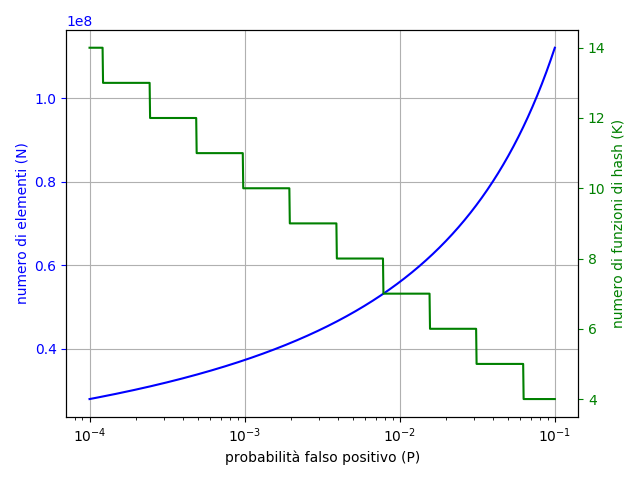
\includegraphics[width=280px]{bloom_parms_1}
	\subcaption{Numero di elementi in base alla probabilità attesa}
	\end{subfigure}

	\begin{subfigure}[t]{280px}
	\centering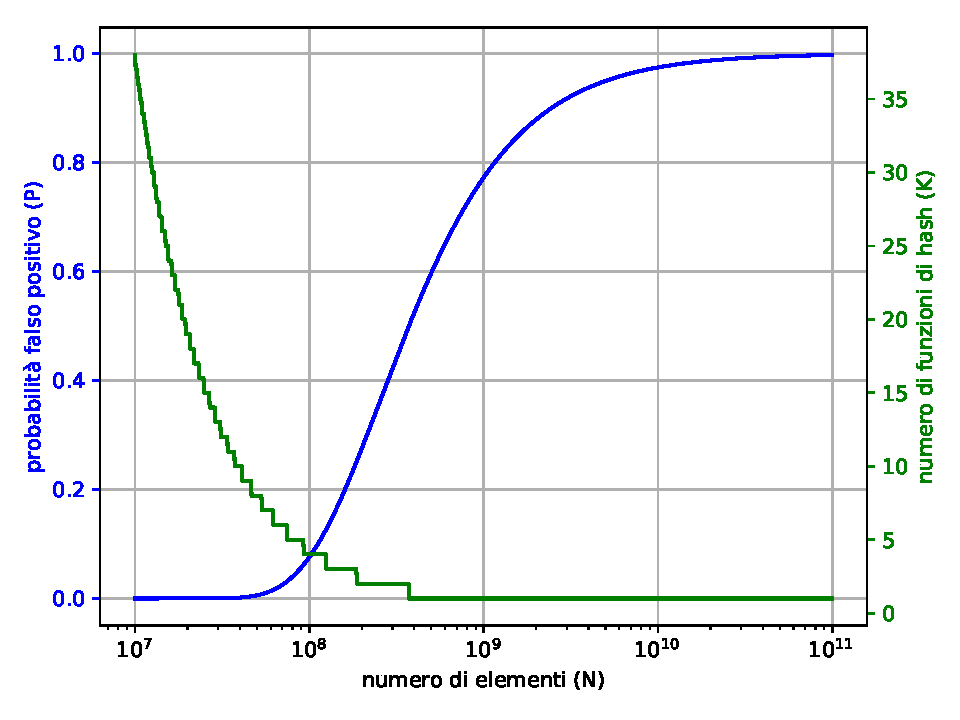
\includegraphics[width=280px]{bloom_parms_2}
	\subcaption{Probabilità attesa in base al numero di elementi}
	\end{subfigure}

	\caption{Andamento dei parametri ottimale in un filtro di 64 MiB}
\end{figure}








